\section{Observaciones}\label{sec:observaciones}

\subsection{Nebulosa de Orión}

Se observa la nebulosa de Orión (ver figura \ref{fig:m42}), también conocida como M42 por su identificación en el catálogo Messier. Esta es una nebulosa difusa situada al sur del cinturón de Orión (ver figura \ref{fig:lb}).
La nebulosa de Orión, también conocida como Messier 42, M42, o NGC 1976, es una nebulosa difusa situada al sur del cinturón de Orión. Tiene un radio de \SI{1.2}{\lightyear} y su distancia a la Tierra es de \SI{1344}{\lightyear}, por lo que es muy cercana y eso la convierte en una buena referencia. Además, en ella hay formación de estrellas de alta masa y también variadas moléculas y partículas, encontrando sus abundancias en \textit{surveys}.

\begin{figure}[p]
	\centering
	\includegraphics[width=3.25in]{rsc/m42.jpg}
	\caption{Nebulosa de Orión (Imagen: NASA)}
	\label{fig:m42}
\end{figure}

\begin{figure}[p]
	\centering
	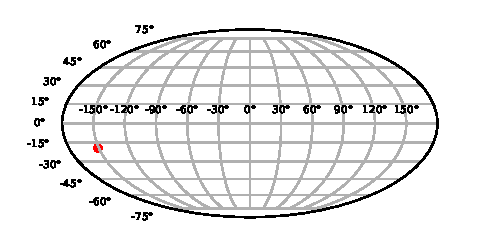
\includegraphics{rsc/lb.pdf}
	\caption{Coordenadas galácticas de la nebulosa de Orión}
	\label{fig:lb}
\end{figure}

Antes de la observación se hace la calibración del telescopio mediante el Hot--Cold Test y Antenna Dipping, tal como se explican en las secciones \ref{sec:hotcoldtest} y \ref{sec:antennadipping}, respectivamente. Esto es importante para tener observaciones más precisas.

Se hace una cruz en el cielo alrededor y centrada en la fuente, tal como muestra la figura \ref{fig:cruz}. Se apunta en el siguiente orden respecto a la figura: arriba, izquierda, centro, derecha y abajo. Esto se repite consecutivamente para un total de 3 pasadas a la cruz.

Los siguientes parámetros se establecen en el software del MINI.

Se usa el modo observacional \textit{position switching}, que necesita definir los puntos: \textit{on pos}, la posición de la fuente; \textit{off pos}, una posición de referencia y; \textit{home pos}, un punto central del mapa que es necesario para calcular la grilla.

Se usa la coordenada ecuatorial de la nebulosa de Orión RA=\ra{5;32;47} y DEC=\ang{-5;24;30} para \textit{on pos} y \textit{home pos}, mientras que para \textit{off pos} se usa RA=\ra{5;40;47} y DEC=\ang{-5;10;0}.

El ciclo \textit{on--off} es de \SI{30}{\second} en total y \SI{15}{\second} por cada posición

El tiempo de integración es \SI{600}{\second}, por lo que el tiempo de observación es el doble.

Además, constantemente se asigna un tiempo de calibración de \SI{5}{\second} para chequear que la atmósfera no ha cambiado respecto al modelo. El espectro obtenido se normaliza al continuo.

\begin{figure}[p]
	\centering
	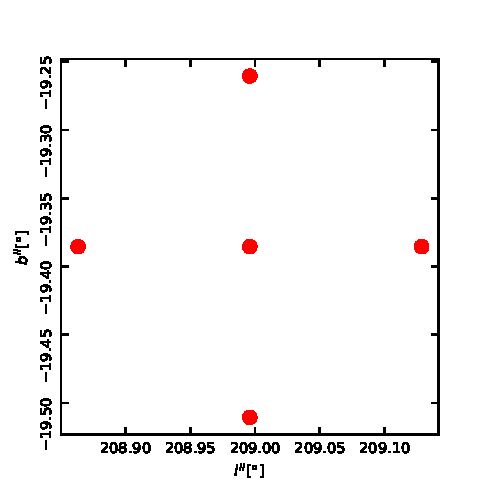
\includegraphics{rsc/cruz.pdf}
	\caption{Cruz de observación}
	\label{fig:cruz}
\end{figure}

El procedimiento para el análisis de las observaciones se muestra en el código \ref{cod:observaciones} y se detalla a continuación.

\subsection{Espectros}

La observación registra los datos provistos por el equipo docente en los archivos \texttt{sdf\_1xx\_1xx}, donde \texttt{xx} va en orden creciente \texttt{11} a \texttt{25}, según el orden de observación de la cruz explicado anteriormente. 

Se miden 256 temperatura en kelvin a distintas velocidades, formando un espectro con una preponderante línea de emisión aproximadamente \SI{9.5}{\kilo\meter\per\second} a aproximadamente \SI{30}{\kelvin} para el punto central. Se hace un ajuste gaussiano para cada uno de estos espectros y se grafica en las figuras \ref{fig:specfit1}, \ref{fig:specfit2} y \ref{fig:specfit3}, para la primera, segunda y tercera pasada por la cruz, respectivamente.

\begin{figure}[p]
	\centering
	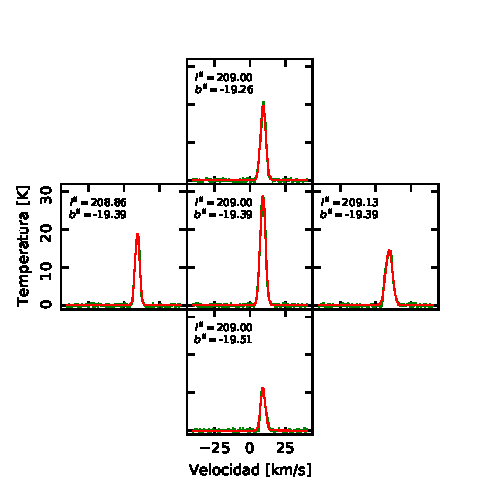
\includegraphics{rsc/specfit1.pdf}
	\caption{Gráfico del espectro y su ajuste gaussiano, primera pasada por la cruz. Línea verde es espectro original. Línea roja es ajuste.}
	\label{fig:specfit1}
\end{figure}

\begin{figure}[p]
	\centering
	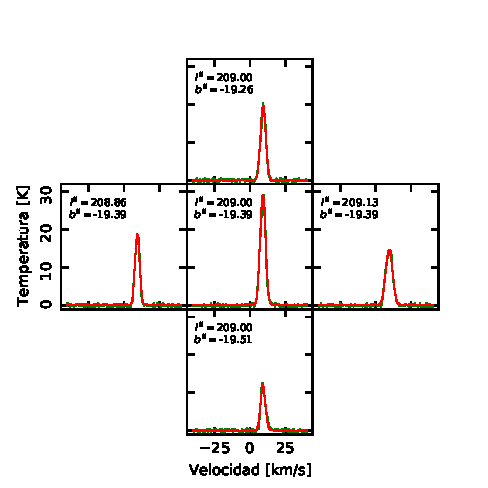
\includegraphics{rsc/specfit2.pdf}
	\caption{Gráfico del espectro y su ajuste gaussiano, segunda pasada por la cruz. Línea verde es espectro original. Línea roja es ajuste.}
	\label{fig:specfit2}
\end{figure}

\begin{figure}[p]
	\centering
	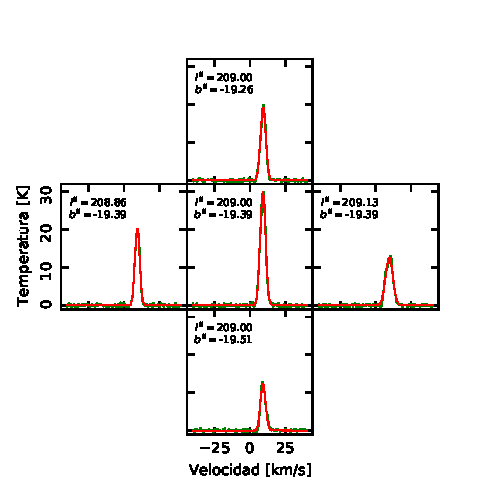
\includegraphics{rsc/specfit3.pdf}
	\caption{Gráfico del espectro y su ajuste gaussiano, tercera pasada por la cruz. Línea verde es espectro original. Línea roja es ajuste.}
	\label{fig:specfit3}
\end{figure}

\subsection{Temperatura máxima y Pointing}

Se calcula la temperatura máxima del espectro para cada una de las quince observaciones. Se promedian las temperaturas correspondientes a las mismas coordenadas en la cruz y se realizan dos ajustes gaussianos, tal como muestra la figura \ref{fig:tmax}. El primer ajuste es a través de la longitud galáctica, manteniendo la latitud galáctica fija, es decir, sobre los tres puntos horizontales de la cruz. El segundo ajuste es a través de la latitud galáctica, manteniendo la longitud galáctica fija, es decir, sobre los tres puntos verticales de la cruz.

El punto central de la cruz tiene una temperatura máxima de \SI{29.215}{\kelvin} a longitud galáctica \SI{208.006}{\degree} y latitud galáctica \SI{-19.385}{\degree}, mientras que el modelo del ajuste gaussiano a latitud fija establece un máximo de \SI{29.485}{\kelvin} a longitud \SI{208.975}{\degree} y el ajuste gaussiano a longitud fija establece un máximo de \SI{29.989}{\kelvin} a latitud \SI{-19.357}{\degree}.

A pesar de que el telescopio tenía ordenado apuntar a la coordenada precisa de la nebulosa de Orión, existe un error que se puede calibrar. Además, el software del telescopio tiene una ventana de tracking que muestra que tiene permitido apuntar dentro de un radio de tolerancia de la coordenada objetivo.

\subsection{Temperatura integrada}

La temperatura integrada en velocidad permite obtener $W_\textnormal{CO}$, que es proporcional a la densidad de columna de hidrógeno molecular, que permite calcular la masa total de una nube molecular compuesta mayoritariamente de hidrógeno.

Se calcula la temperatura integrada del espectro para cada una de las quince observaciones. Se promedian las temperaturas correspondientes a las mismas coordenadas en la cruz y se realizan dos ajustes gaussianos, tal como muestra la figura \ref{fig:tint}. El primer ajuste es a través de la longitud galáctica, manteniendo la latitud galáctica fija, es decir, sobre los tres puntos horizontales de la cruz. El segundo ajuste es a través de la latitud galáctica, manteniendo la longitud galáctica fija, es decir, sobre los tres puntos verticales de la cruz.

\begin{figure}[h]
	\centering
	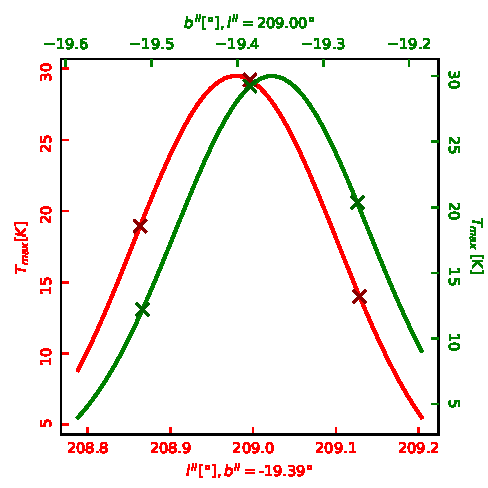
\includegraphics{rsc/tmax.pdf}
	\caption{Gráfico de temperatura máxima y su ajuste gaussiano. Línea roja es ajuste de los puntos a latitud fija y se mide en los ejes inferior e izquierdo. Línea verde es ajuste de los puntos a longitud fija y se mide en los ejes superior y derecho. Equis roja es medición en la cruz, en orden creciente de longitud: punto de arriba, centro y abajo. Equis verde es medición en la cruz, en orden creciente de latitud: punto de izquierda, centro y derecha.}
	\label{fig:tmax}
\end{figure}

\begin{figure}[h]
	\centering
	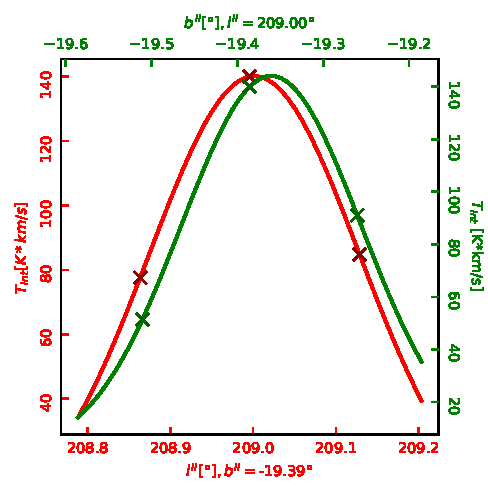
\includegraphics{rsc/tint.pdf}
	\caption{Gráfico de temperatura integrada y su ajuste gaussiano. Línea roja es ajuste de los puntos a latitud fija y se mide en los ejes inferior e izquierdo. Línea verde es ajuste de los puntos a longitud fija y se mide en los ejes superior y derecho. Equis roja es medición en la cruz, en orden creciente de longitud: punto de arriba, centro y abajo. Equis verde es medición en la cruz, en orden creciente de latitud: punto de izquierda, centro y derecha.}
	\label{fig:tint}
\end{figure}

\subsection{Error RMS y comparación}

Sea $\Delta T_\textnormal{A}$ el error total para $N$ muestras promediadas, $T_\textnormal{sys}$ el error para una única muestra, $\tau$ el tiempo total, $\Delta\nu$ el ancho de banda. La estadística gaussiana establece la siguiente relación entre el error para las muestras promediadas y el error para una única muestra,
\begin{equation}
\Delta T_\textnormal{A}=\frac{T_\textnormal{sys}}{\sqrt{N}}=\frac{T_\textnormal{sys}}{\sqrt{\tau\Delta\nu}}\label{eq:rms1}
,\end{equation}
pero en la práctica hay un factor $C_\textnormal{obs}$ que depende del modo de observación,
\begin{equation}
\Delta T_\textnormal{A}=\frac{C_\textnormal{obs}T_\textnormal{sys}}{\sqrt{N}}=\frac{C_\textnormal{obs}T_\textnormal{sys}}{\sqrt{\tau\Delta\nu}}\label{eq:rms2}
,\end{equation}
donde la constante observacional $C_\textnormal{obs}$ para el modo \textit{position switching}, que apunta tanto a la fuente como fuera de esta, es igual a $\sqrt{2}$.

Por un lado, se utiliza la técnica de \textit{sigma clipping} para obtener la base de ruido de los espectros y eliminar la línea de emisión para el siguiente cálculo, utilizando $\sigma=3$ y las iteraciones necesarias hasta que el algoritmo converja. Se calcula el error RMS del ruido para cada uno de los quince espectros.

Por otro lado, se promedian los espectros correspondientes a la misma coordenada en la cruz. Se les aplica la técnica de \textit{sigma clipping} con los mismos parámetros anteriores. Se calcula el error RMS del ruido para cada uno de los cinco nuevos espectros.

Los resultados se muestran en la tabla \ref{tab:rms}, que tiene los valores $\Delta T_\textnormal{A}/T_\textnormal{sys}$.

La ecuación \ref{eq:rms1} y la cantidad de datos promediados establecen que el cuociente teórico entre el error del promedio y el error de una muestra única es $1/\sqrt{3}=0.577$, pero si se considera la constante observacional entonces es $\sqrt{2}/\sqrt{3}=0.816$.

\begin{table*}[htbp]
	\centering
	\begin{tabular}{
			@{}
			l
			S[table-format=2.3]
			S[table-format=2.3]
			S[table-format=2.3]
			S[table-format=2.3]
			S[table-format=2.3]
			@{}
		}
		\toprule
		{Pasada} &
		{Arriba} &
		{Izquierda} &
		{Centro} &
		{Derecha} &
		{Abajo} \\
		\midrule
		Primera & 0.583 & 0.573 & 0.579 & 0.555 & 0.552 \\
		Segunda & 0.621 & 0.601 & 0.640 & 0.628 & 0.593 \\
		Tercera & 0.637 & 0.619 & 0.626 & 1.084 & 0.599 \\
		\bottomrule
	\end{tabular}
	\caption{Cociente entre error de los puntos de la cruz promediados y error de los puntos sin promediar}\label{tab:rms}
\end{table*}

